\section{external\_\-flash.h File Reference}
\label{external__flash_8h}\index{external_flash.h@{external\_\-flash.h}}


This graph shows which files directly or indirectly include this file:\begin{figure}[H]
\begin{center}
\leavevmode
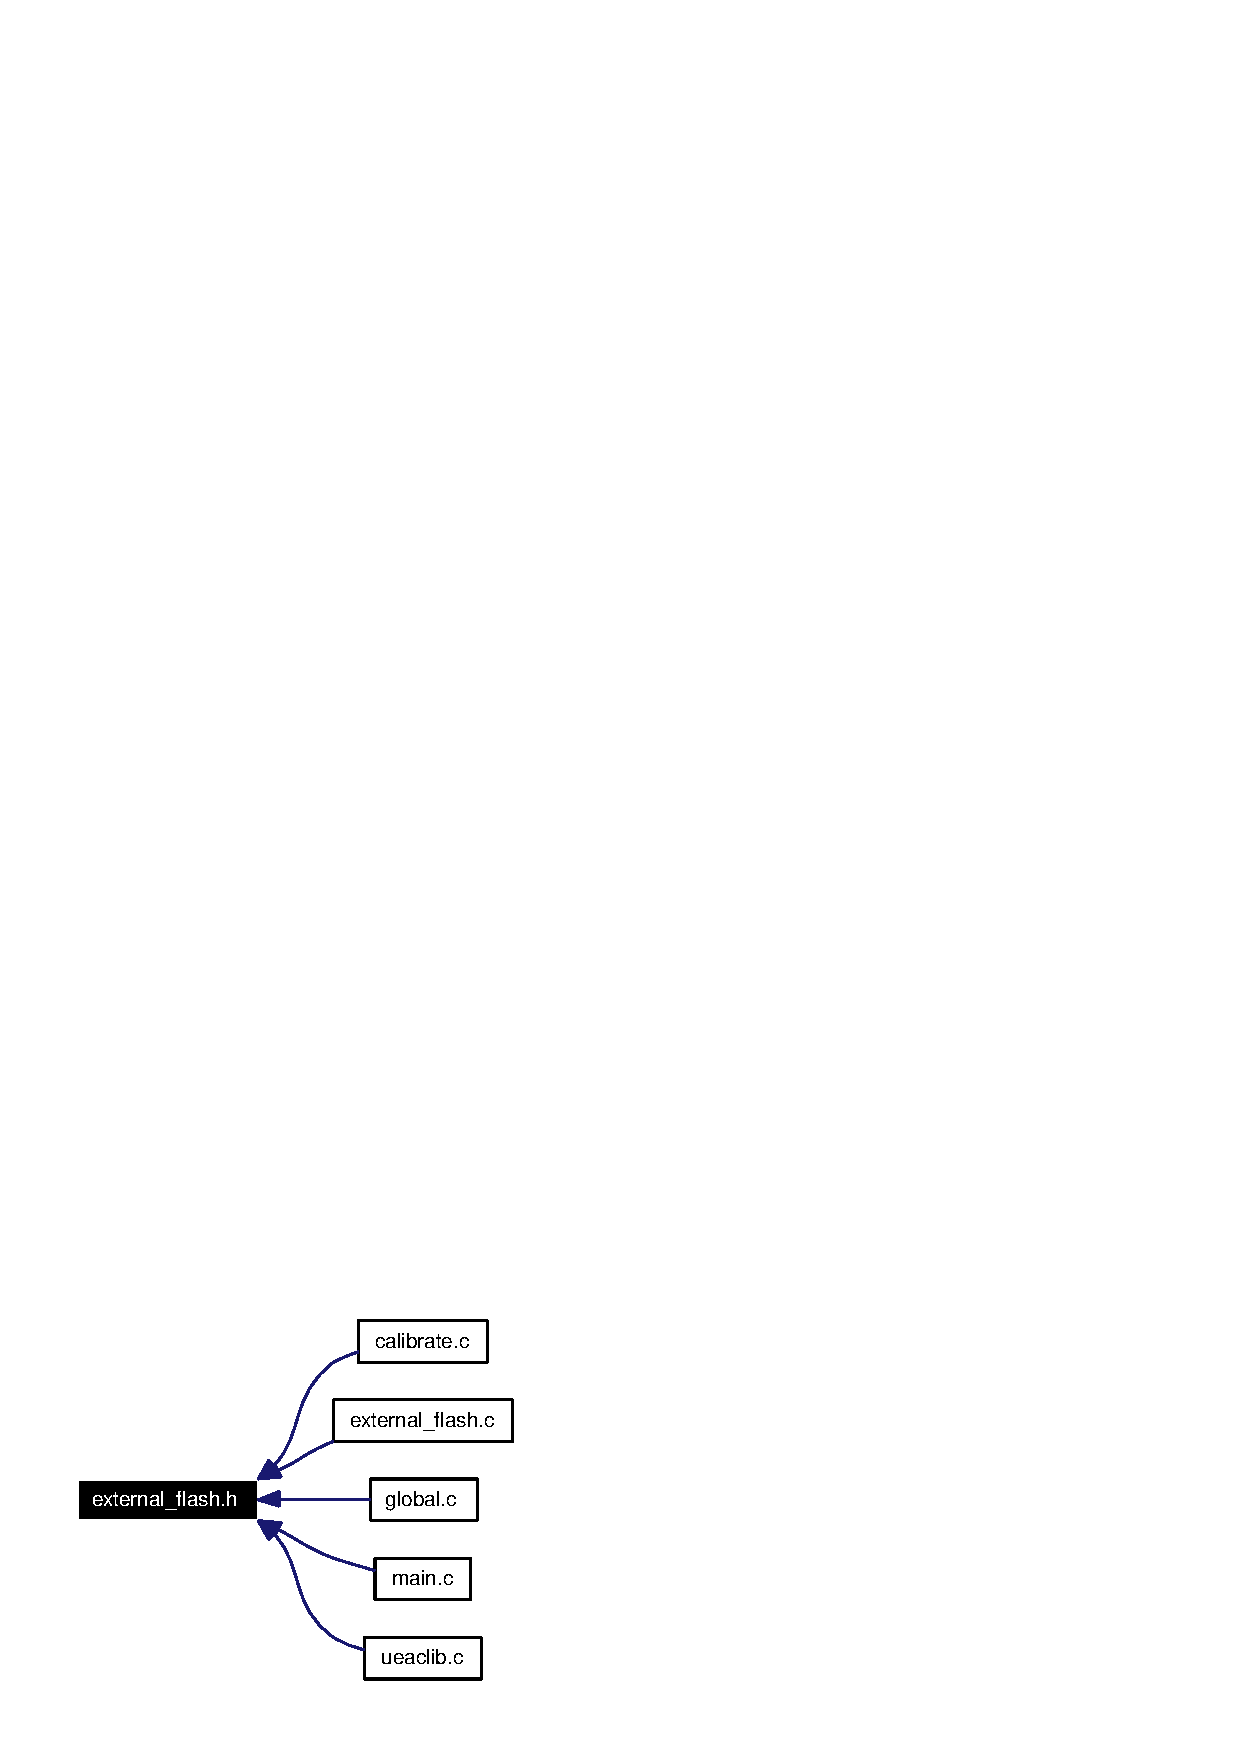
\includegraphics[width=123pt]{external__flash_8h__dep__incl}
\end{center}
\end{figure}
\subsection*{Defines}
\begin{CompactItemize}
\item 
\#define {\bf n\-CS\_\-LOW}~\{P4OUT \&= $\sim$BIT3;\}
\item 
\#define {\bf n\-CS\_\-HIGH}~\{P4OUT $|$= BIT3;\}
\item 
\#define {\bf PAGE\_\-SIZE}~264
\item 
\#define {\bf NUMBER\_\-PAGES}~1024
\end{CompactItemize}
\subsection*{Functions}
\begin{CompactItemize}
\item 
int {\bf flash\_\-integrity\_\-test} (void)
\item 
unsigned char {\bf send\_\-spi\_\-byte} (unsigned char)
\item 
void {\bf init\_\-spi} (void)
\item 
void {\bf start\_\-main\_\-array\_\-read} (unsigned short, unsigned short)
\item 
void {\bf end\_\-main\_\-array\_\-read} (void)
\item 
void {\bf page\_\-to\_\-buffer1\_\-compare} (unsigned short)
\item 
void {\bf buffer1\_\-to\_\-page\_\-e} (unsigned short)
\item 
void {\bf buffer2\_\-to\_\-page\_\-e} (unsigned short)
\item 
unsigned char {\bf poll\_\-status\_\-register\_\-blocking} (void)
\item 
void {\bf buffer1\_\-write} (unsigned short, unsigned char)
\item 
void {\bf buffer2\_\-write} (unsigned short, unsigned char)
\item 
unsigned char {\bf buffer1\_\-read} (unsigned short)
\item 
unsigned char {\bf buffer2\_\-read} (unsigned short)
\end{CompactItemize}


\subsection{Define Documentation}
\index{external_flash.h@{external\_\-flash.h}!nCS_HIGH@{nCS\_\-HIGH}}
\index{nCS_HIGH@{nCS\_\-HIGH}!external_flash.h@{external\_\-flash.h}}
\subsubsection{\setlength{\rightskip}{0pt plus 5cm}\#define n\-CS\_\-HIGH~\{P4OUT $|$= BIT3;\}}\label{external__flash_8h_a1}




Definition at line 60 of file external\_\-flash.h.

Referenced by buffer1\_\-read(), buffer1\_\-to\_\-page\_\-e(), buffer1\_\-write(), buffer2\_\-read(), buffer2\_\-to\_\-page\_\-e(), buffer2\_\-write(), end\_\-main\_\-array\_\-read(), page\_\-to\_\-buffer1\_\-compare(), and poll\_\-status\_\-register\_\-blocking().\index{external_flash.h@{external\_\-flash.h}!nCS_LOW@{nCS\_\-LOW}}
\index{nCS_LOW@{nCS\_\-LOW}!external_flash.h@{external\_\-flash.h}}
\subsubsection{\setlength{\rightskip}{0pt plus 5cm}\#define n\-CS\_\-LOW~\{P4OUT \&= $\sim$BIT3;\}}\label{external__flash_8h_a0}




Definition at line 59 of file external\_\-flash.h.

Referenced by buffer1\_\-read(), buffer1\_\-to\_\-page\_\-e(), buffer1\_\-write(), buffer2\_\-read(), buffer2\_\-to\_\-page\_\-e(), buffer2\_\-write(), page\_\-to\_\-buffer1\_\-compare(), poll\_\-status\_\-register\_\-blocking(), and start\_\-main\_\-array\_\-read().\index{external_flash.h@{external\_\-flash.h}!NUMBER_PAGES@{NUMBER\_\-PAGES}}
\index{NUMBER_PAGES@{NUMBER\_\-PAGES}!external_flash.h@{external\_\-flash.h}}
\subsubsection{\setlength{\rightskip}{0pt plus 5cm}\#define NUMBER\_\-PAGES~1024}\label{external__flash_8h_a3}




Definition at line 62 of file external\_\-flash.h.\index{external_flash.h@{external\_\-flash.h}!PAGE_SIZE@{PAGE\_\-SIZE}}
\index{PAGE_SIZE@{PAGE\_\-SIZE}!external_flash.h@{external\_\-flash.h}}
\subsubsection{\setlength{\rightskip}{0pt plus 5cm}\#define PAGE\_\-SIZE~264}\label{external__flash_8h_a2}




Definition at line 61 of file external\_\-flash.h.

Referenced by current\_\-output\_\-calibration(), and flash\_\-integrity\_\-test().

\subsection{Function Documentation}
\index{external_flash.h@{external\_\-flash.h}!buffer1_read@{buffer1\_\-read}}
\index{buffer1_read@{buffer1\_\-read}!external_flash.h@{external\_\-flash.h}}
\subsubsection{\setlength{\rightskip}{0pt plus 5cm}unsigned char buffer1\_\-read (unsigned {\em short})}\label{external__flash_8h_a15}




Definition at line 244 of file external\_\-flash.c.

References n\-CS\_\-HIGH, n\-CS\_\-LOW, and send\_\-spi\_\-byte().

Referenced by flash\_\-integrity\_\-test().

\footnotesize\begin{verbatim}244                                                 {
245   unsigned char temp;
246   nCS_LOW;
247   send_spi_byte(0xD4);       // command for byte write to buff 1
248   send_spi_byte(0x00);       // dummy byte
249   if (addr>0xFF) {
250     send_spi_byte(0x01);     // MSB of buffer address
251   }
252   else {
253     send_spi_byte(0x00);     // MSB of buffer address
254   }  
255   send_spi_byte((unsigned char) addr); // send the balance of the address
256   send_spi_byte(0x00);       // extra clocks required by the flash
257   temp=send_spi_byte(0x00);  // this is the data 
258   nCS_HIGH; 
259   return(temp);
260 }
\end{verbatim}\normalsize 




Here is the call graph for this function:\begin{figure}[H]
\begin{center}
\leavevmode
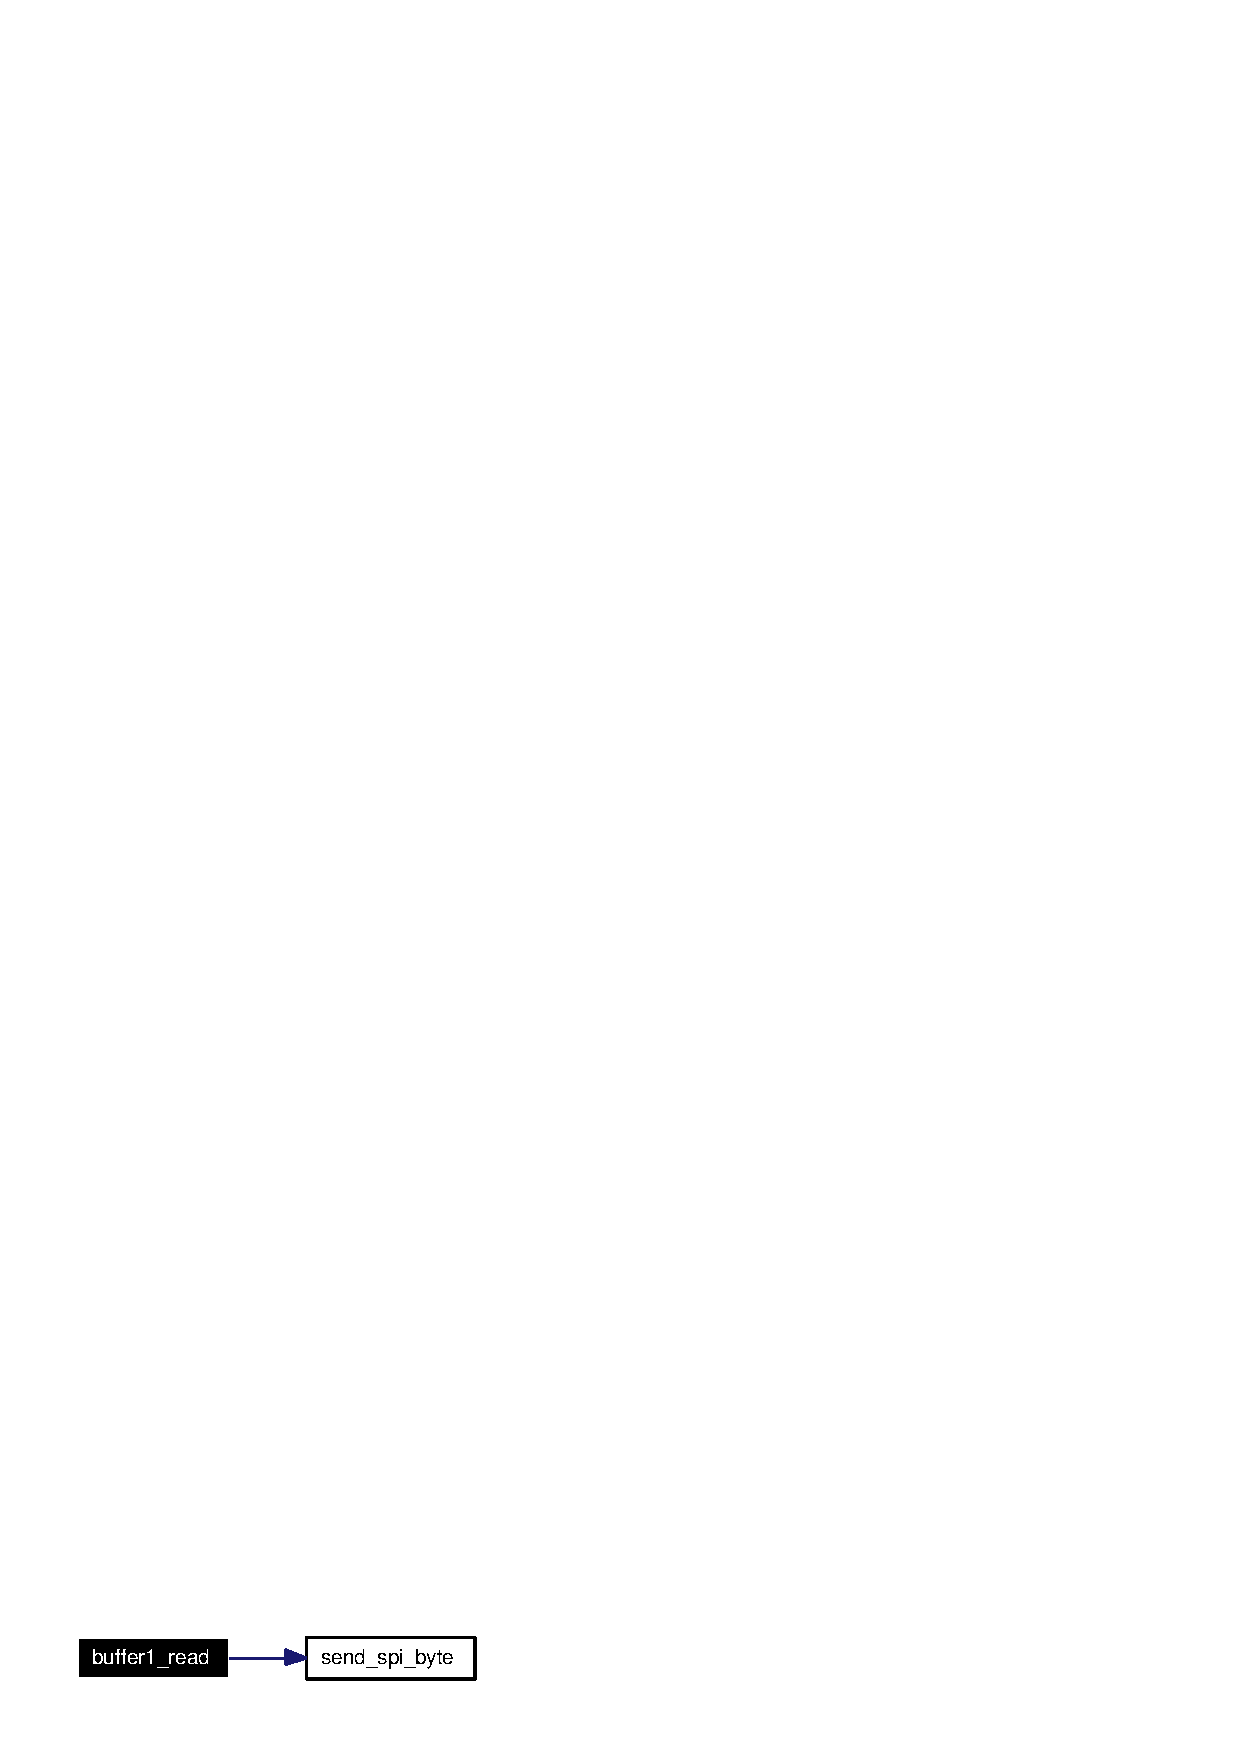
\includegraphics[width=114pt]{external__flash_8h_a15_cgraph}
\end{center}
\end{figure}
\index{external_flash.h@{external\_\-flash.h}!buffer1_to_page_e@{buffer1\_\-to\_\-page\_\-e}}
\index{buffer1_to_page_e@{buffer1\_\-to\_\-page\_\-e}!external_flash.h@{external\_\-flash.h}}
\subsubsection{\setlength{\rightskip}{0pt plus 5cm}void buffer1\_\-to\_\-page\_\-e (unsigned {\em short})}\label{external__flash_8h_a10}




Definition at line 177 of file external\_\-flash.c.

References n\-CS\_\-HIGH, n\-CS\_\-LOW, and send\_\-spi\_\-byte().

Referenced by current\_\-output\_\-calibration().

\footnotesize\begin{verbatim}177                                             {
178   unsigned char page_temp;
179   nCS_LOW;
180   send_spi_byte(0x83);       // 0x83 command for byte write to buff 1
181   page_temp = (unsigned char)(page>>7);
182   send_spi_byte (page_temp);
183   page_temp = (unsigned char) (page<<1);
184   send_spi_byte (page_temp);
185   send_spi_byte (0x00);
186   nCS_HIGH;                 // starts the page erase and program 
187 }
\end{verbatim}\normalsize 




Here is the call graph for this function:\begin{figure}[H]
\begin{center}
\leavevmode
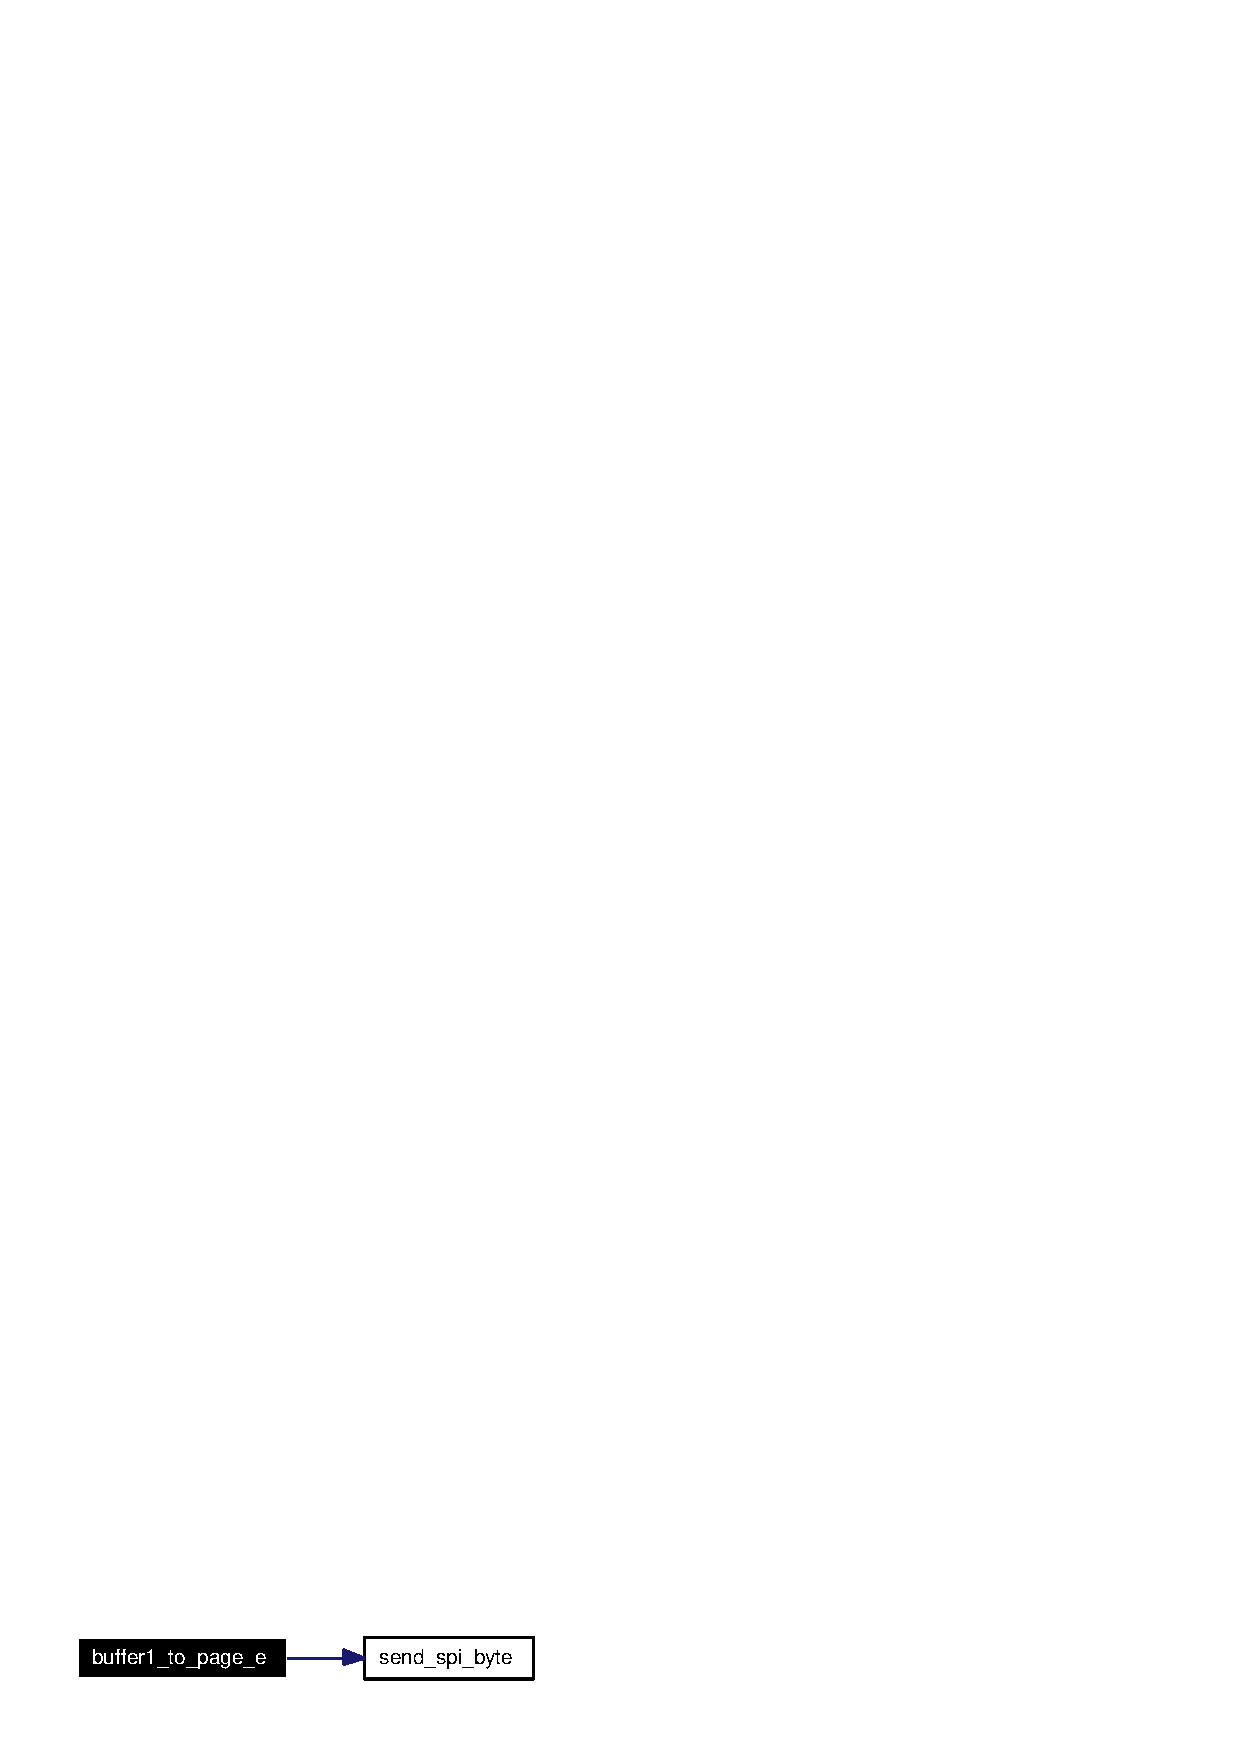
\includegraphics[width=128pt]{external__flash_8h_a10_cgraph}
\end{center}
\end{figure}
\index{external_flash.h@{external\_\-flash.h}!buffer1_write@{buffer1\_\-write}}
\index{buffer1_write@{buffer1\_\-write}!external_flash.h@{external\_\-flash.h}}
\subsubsection{\setlength{\rightskip}{0pt plus 5cm}void buffer1\_\-write (unsigned {\em short}, unsigned {\em char})}\label{external__flash_8h_a13}




Definition at line 214 of file external\_\-flash.c.

References n\-CS\_\-HIGH, n\-CS\_\-LOW, and send\_\-spi\_\-byte().

Referenced by current\_\-output\_\-calibration(), and flash\_\-integrity\_\-test().

\footnotesize\begin{verbatim}214                                                                  {
215   nCS_LOW;
216   send_spi_byte(0x84);       // command for byte write to buff 1
217   send_spi_byte(0x00);       // dummy byte
218   if (addr>0xFF) {
219     send_spi_byte(0x01);     // dummy byte except 
220   }
221   else {
222     send_spi_byte(0x00);     // dummy byte except 
223   }  
224   send_spi_byte((unsigned char) addr); // send the balance of the address
225   send_spi_byte(data_byte);
226   nCS_HIGH; 
227 }
\end{verbatim}\normalsize 




Here is the call graph for this function:\begin{figure}[H]
\begin{center}
\leavevmode
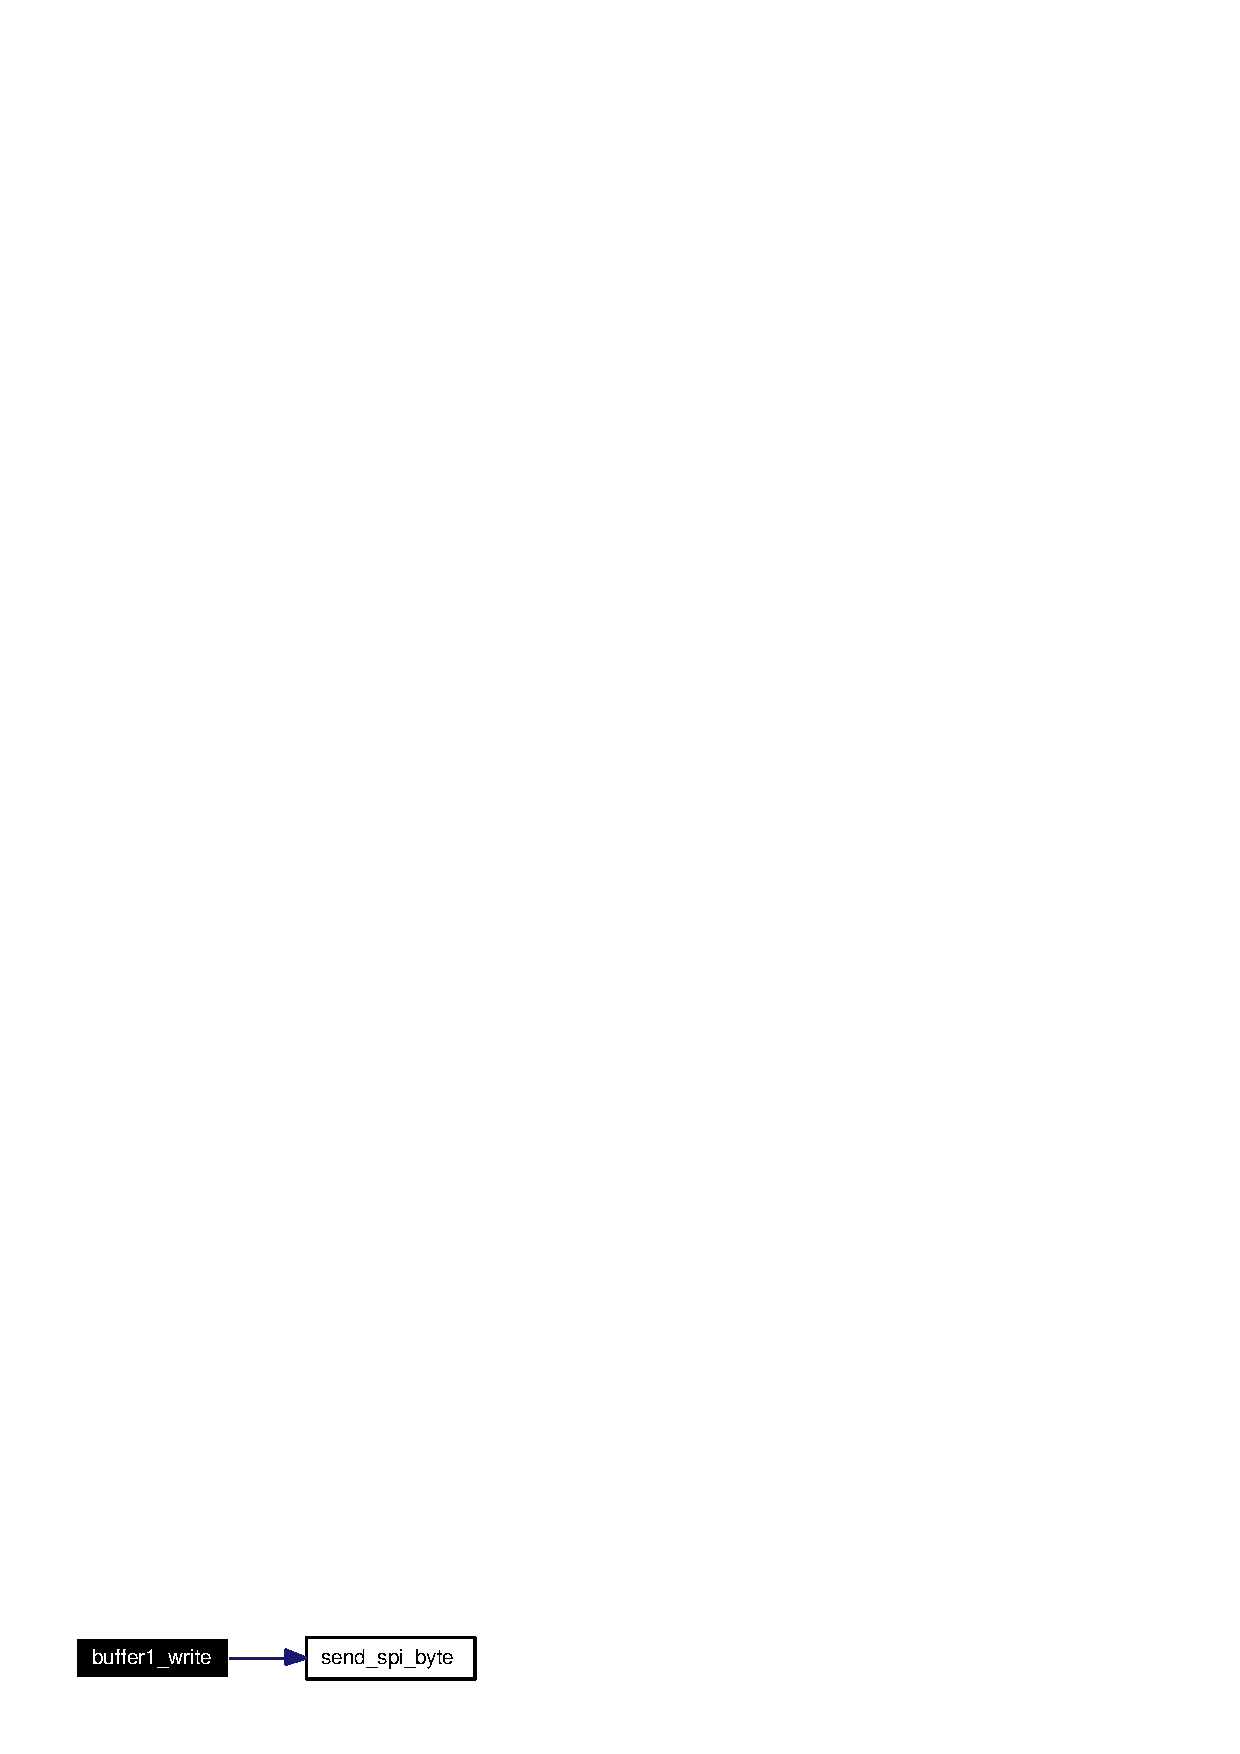
\includegraphics[width=114pt]{external__flash_8h_a13_cgraph}
\end{center}
\end{figure}
\index{external_flash.h@{external\_\-flash.h}!buffer2_read@{buffer2\_\-read}}
\index{buffer2_read@{buffer2\_\-read}!external_flash.h@{external\_\-flash.h}}
\subsubsection{\setlength{\rightskip}{0pt plus 5cm}unsigned char buffer2\_\-read (unsigned {\em short})}\label{external__flash_8h_a16}




Definition at line 262 of file external\_\-flash.c.

References n\-CS\_\-HIGH, n\-CS\_\-LOW, and send\_\-spi\_\-byte().

Referenced by flash\_\-integrity\_\-test().

\footnotesize\begin{verbatim}262                                                 {
263   unsigned char temp;
264   nCS_LOW;
265   send_spi_byte(0xD6);       // command for byte write to buff 1
266   send_spi_byte(0x00);       // dummy byte
267   if (addr>0xFF) {
268     send_spi_byte(0x01);     // MSB of buffer address
269   }
270   else {
271     send_spi_byte(0x00);     // MSB of buffer address
272   }  
273   send_spi_byte((unsigned char) addr); // send the balance of the address
274   send_spi_byte(0x00);       // extra clocks required by the flash
275   temp=send_spi_byte(0x00);  // this is the data 
276   nCS_HIGH; 
277   return(temp);
278 }
\end{verbatim}\normalsize 




Here is the call graph for this function:\begin{figure}[H]
\begin{center}
\leavevmode
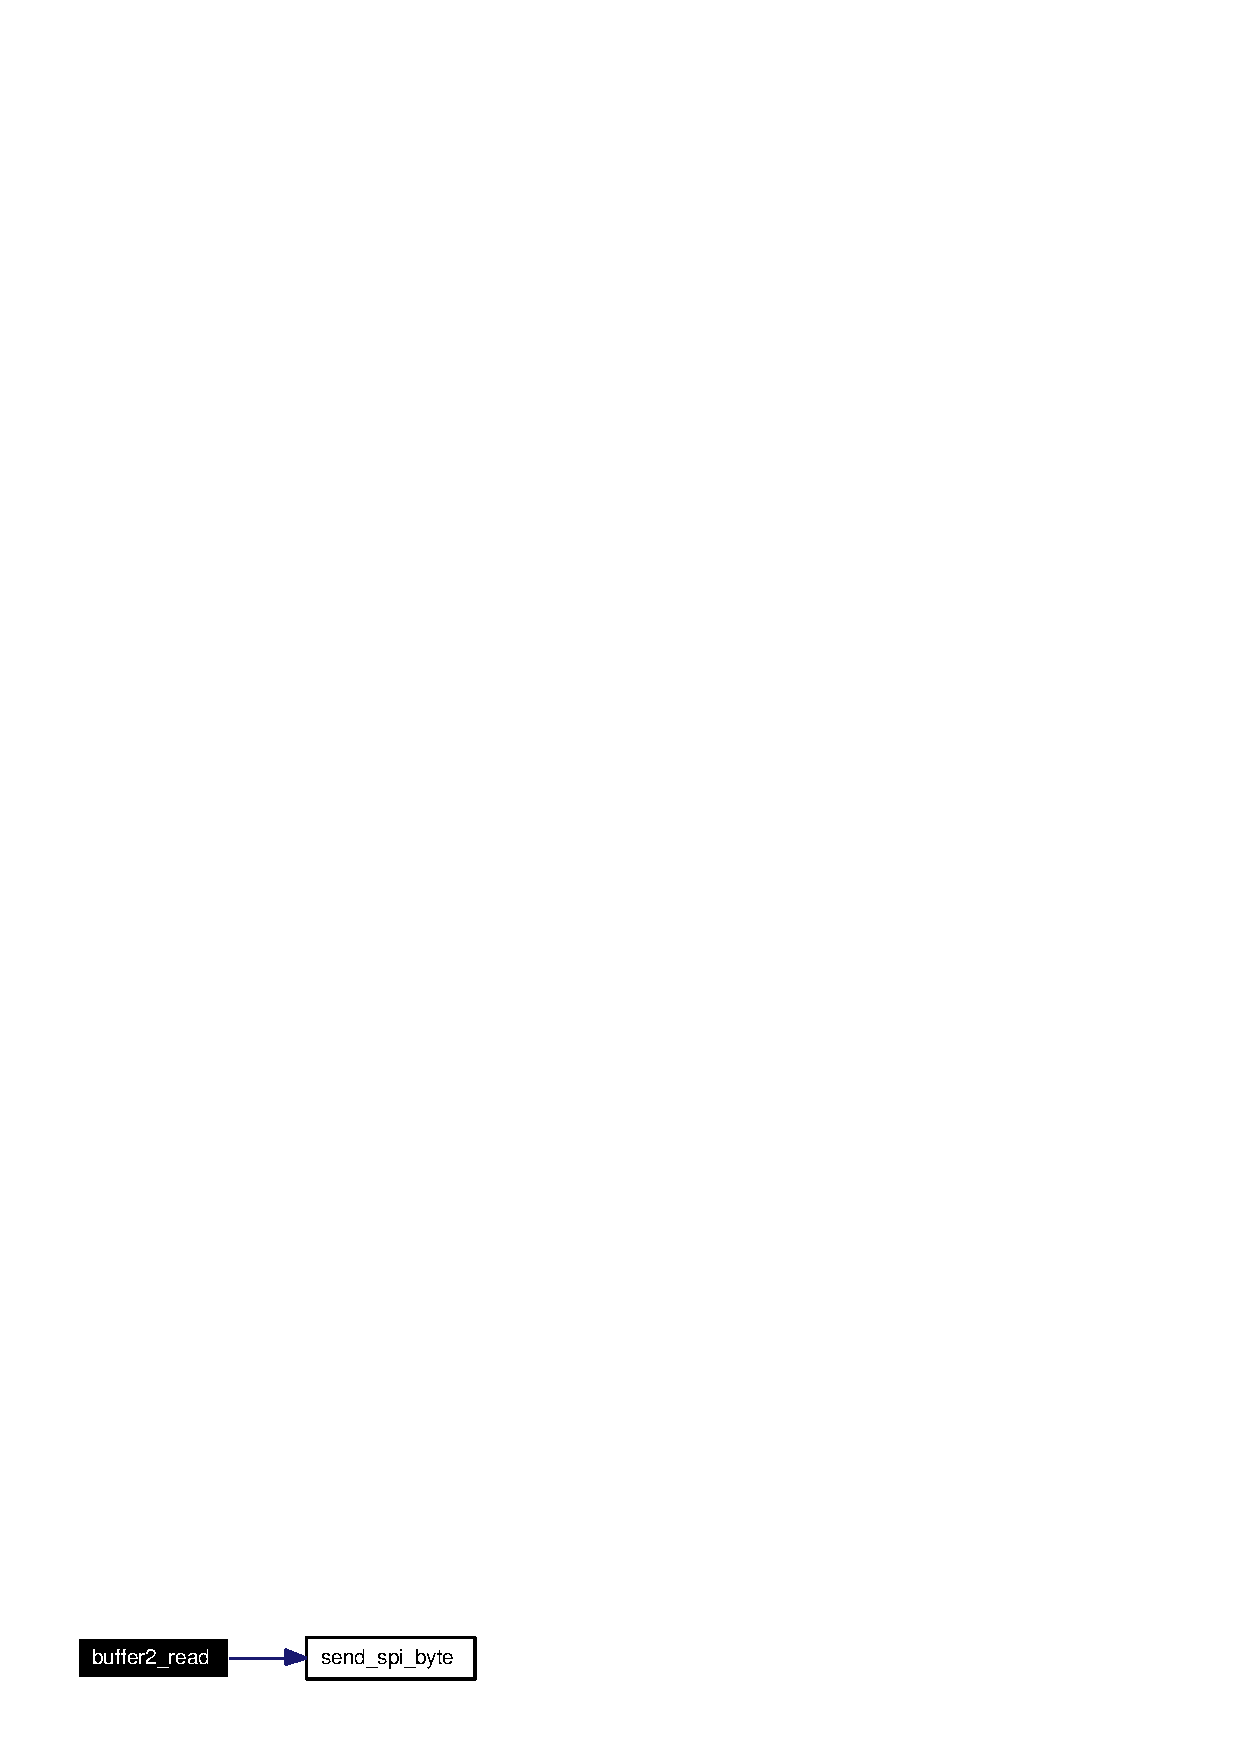
\includegraphics[width=114pt]{external__flash_8h_a16_cgraph}
\end{center}
\end{figure}
\index{external_flash.h@{external\_\-flash.h}!buffer2_to_page_e@{buffer2\_\-to\_\-page\_\-e}}
\index{buffer2_to_page_e@{buffer2\_\-to\_\-page\_\-e}!external_flash.h@{external\_\-flash.h}}
\subsubsection{\setlength{\rightskip}{0pt plus 5cm}void buffer2\_\-to\_\-page\_\-e (unsigned {\em short})}\label{external__flash_8h_a11}




Definition at line 189 of file external\_\-flash.c.

References n\-CS\_\-HIGH, n\-CS\_\-LOW, and send\_\-spi\_\-byte().

\footnotesize\begin{verbatim}189                                             {
190   unsigned char page_temp;
191   nCS_LOW;
192   send_spi_byte(0x86);       // 0x86 command for byte write to buff 2
193   page_temp = (unsigned char)(page>>7);
194   send_spi_byte (page_temp);
195   page_temp = (unsigned char) (page<<1);
196   send_spi_byte (page_temp);
197   send_spi_byte (0x00);
198   nCS_HIGH;                 // starts the page erase and program 
199 }
\end{verbatim}\normalsize 




Here is the call graph for this function:\begin{figure}[H]
\begin{center}
\leavevmode
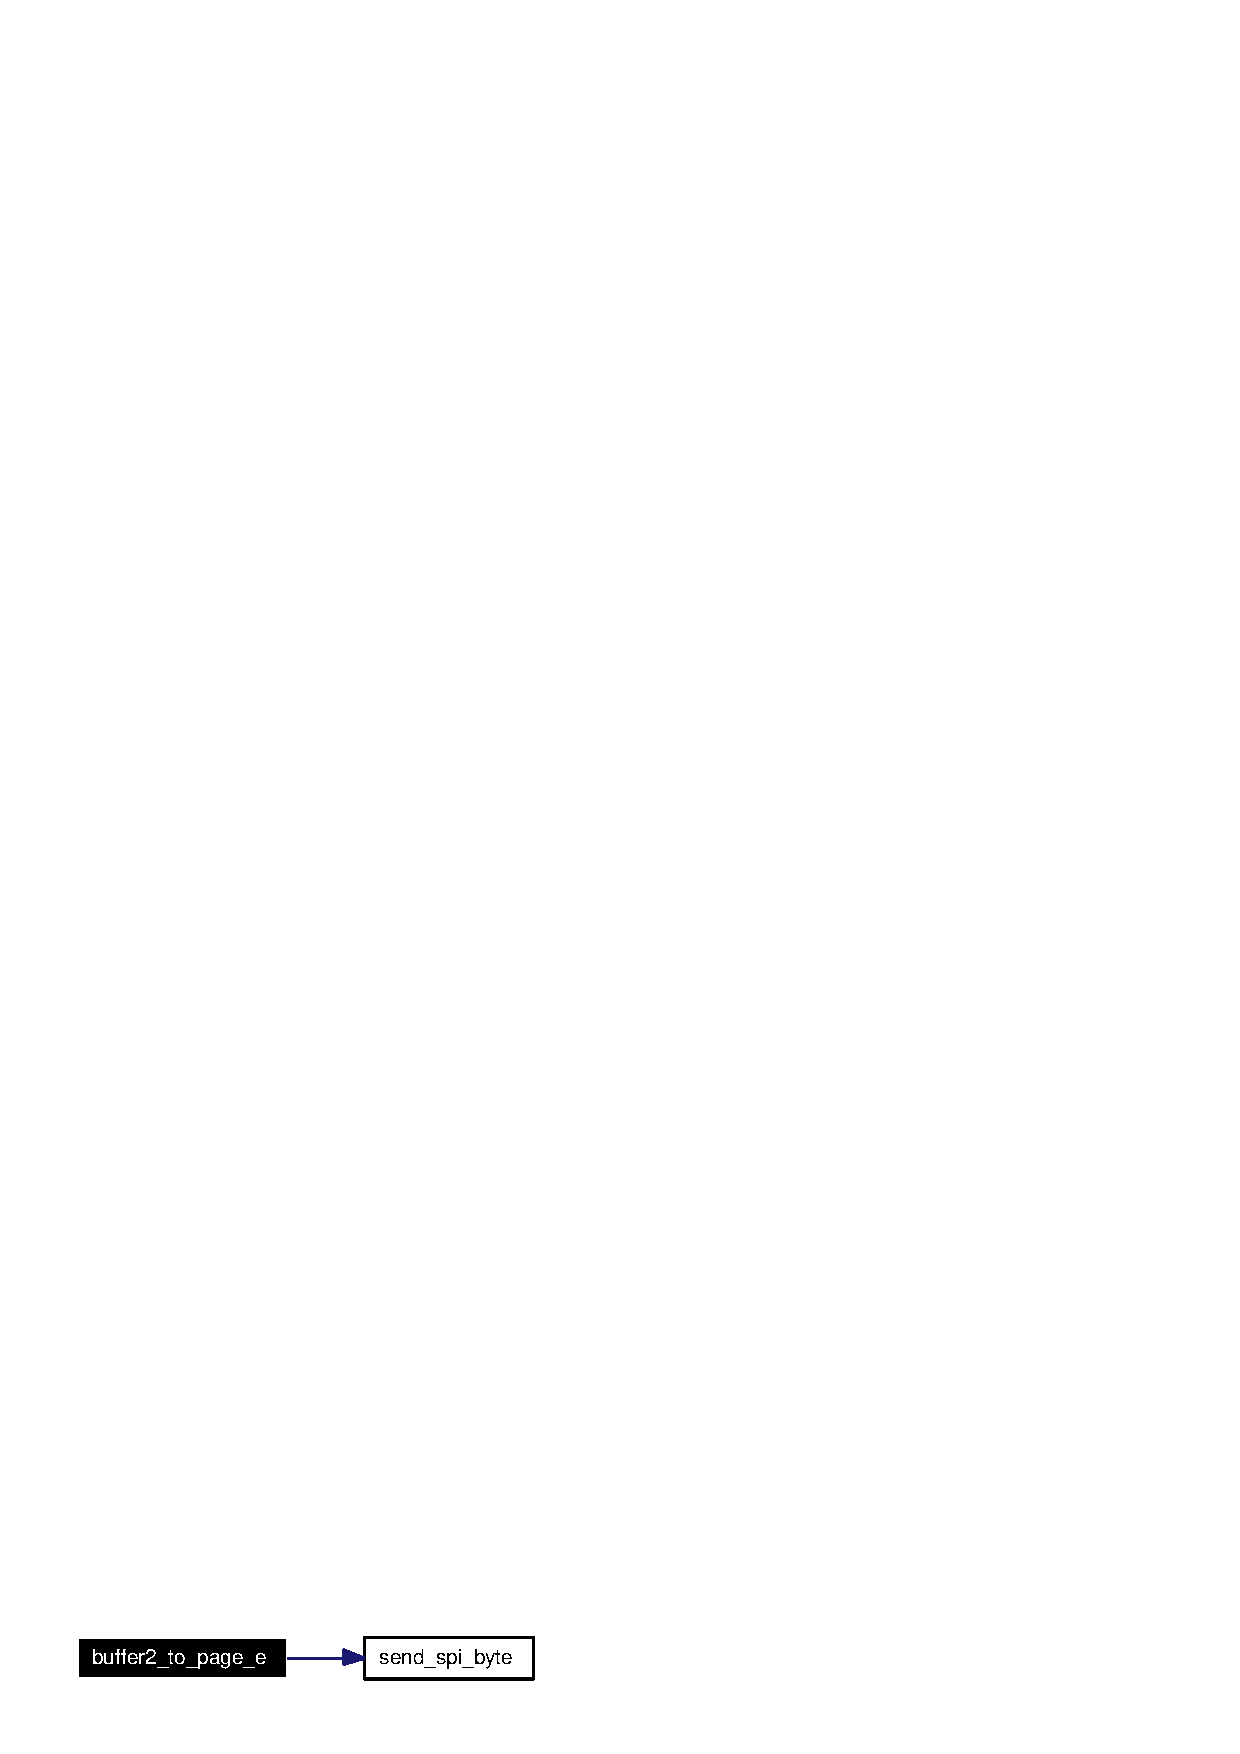
\includegraphics[width=128pt]{external__flash_8h_a11_cgraph}
\end{center}
\end{figure}
\index{external_flash.h@{external\_\-flash.h}!buffer2_write@{buffer2\_\-write}}
\index{buffer2_write@{buffer2\_\-write}!external_flash.h@{external\_\-flash.h}}
\subsubsection{\setlength{\rightskip}{0pt plus 5cm}void buffer2\_\-write (unsigned {\em short}, unsigned {\em char})}\label{external__flash_8h_a14}




Definition at line 229 of file external\_\-flash.c.

References n\-CS\_\-HIGH, n\-CS\_\-LOW, and send\_\-spi\_\-byte().

Referenced by flash\_\-integrity\_\-test().

\footnotesize\begin{verbatim}229                                                                  {
230   nCS_LOW;
231   send_spi_byte(0x87);       // command for byte write to buff 2
232   send_spi_byte(0x00);       // dummy byte
233   if (addr>0xFF) {
234     send_spi_byte(0x01);     // dummy byte except 
235   }
236   else {
237     send_spi_byte(0x00);     // dummy byte except 
238   }  
239   send_spi_byte((unsigned char) addr); // send the balance of the address
240   send_spi_byte(data_byte);
241   nCS_HIGH; 
242 }
\end{verbatim}\normalsize 




Here is the call graph for this function:\begin{figure}[H]
\begin{center}
\leavevmode
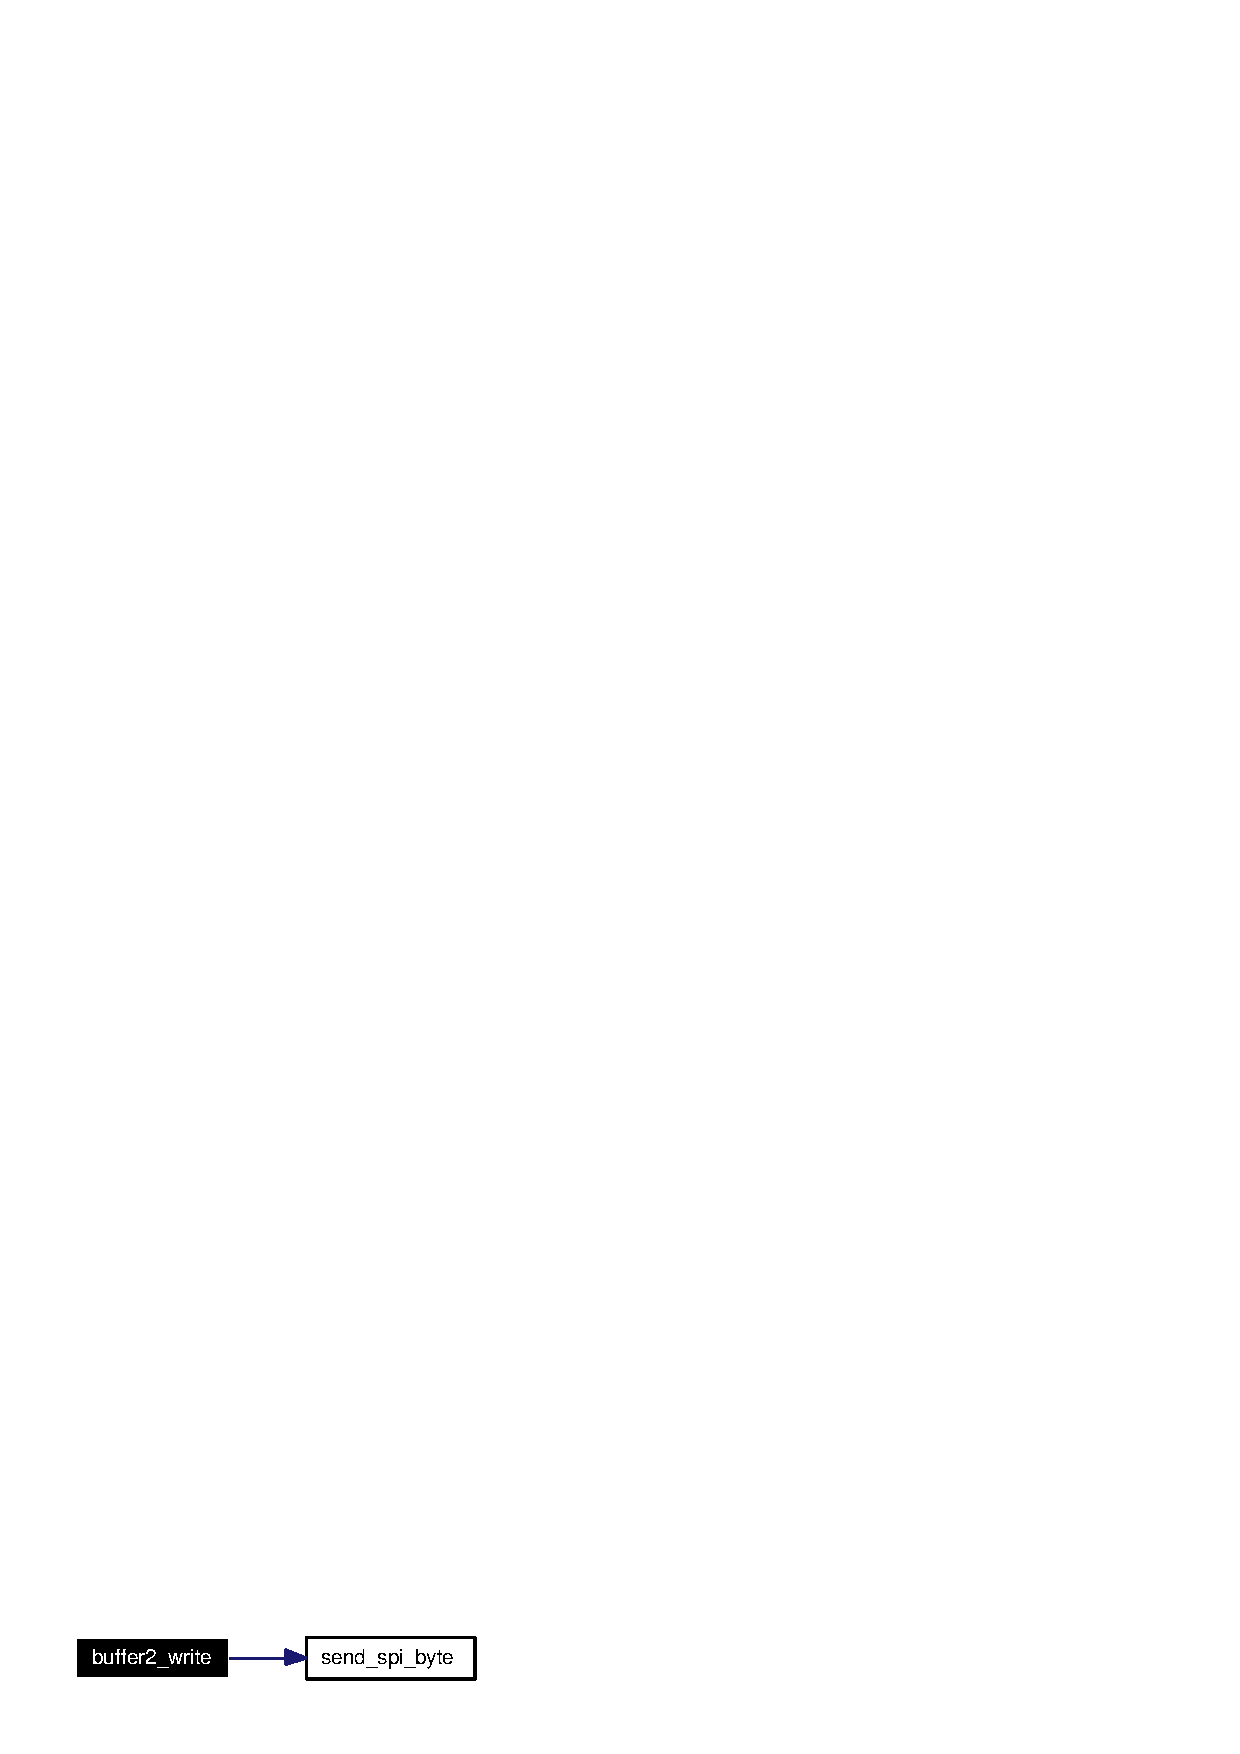
\includegraphics[width=114pt]{external__flash_8h_a14_cgraph}
\end{center}
\end{figure}
\index{external_flash.h@{external\_\-flash.h}!end_main_array_read@{end\_\-main\_\-array\_\-read}}
\index{end_main_array_read@{end\_\-main\_\-array\_\-read}!external_flash.h@{external\_\-flash.h}}
\subsubsection{\setlength{\rightskip}{0pt plus 5cm}void end\_\-main\_\-array\_\-read (void)}\label{external__flash_8h_a8}




Definition at line 161 of file external\_\-flash.c.

References n\-CS\_\-HIGH.

Referenced by init\_\-ueac\_\-state\_\-structure().

\footnotesize\begin{verbatim}161                                {
162   nCS_HIGH;
163 }
\end{verbatim}\normalsize 


\index{external_flash.h@{external\_\-flash.h}!flash_integrity_test@{flash\_\-integrity\_\-test}}
\index{flash_integrity_test@{flash\_\-integrity\_\-test}!external_flash.h@{external\_\-flash.h}}
\subsubsection{\setlength{\rightskip}{0pt plus 5cm}int flash\_\-integrity\_\-test (void)}\label{external__flash_8h_a4}




Definition at line 53 of file external\_\-flash.c.

References BLACK, buffer1\_\-read(), buffer1\_\-write(), buffer2\_\-read(), buffer2\_\-write(), GREEN, PAGE\_\-SIZE, and RED.

Referenced by main().

\footnotesize\begin{verbatim}53                                {
54   enum {PASS,FAIL};
55   int i,fail_flag; 
56   unsigned char data=0;
57   // unsigned short page=0;
58   // printf("### Flash Tests ###\n\r");
59   // SRAM BUFFER 1
60 
61   //  poll_status_register_blocking();                  // Wait for the flash page erase/write to complete 
62   fail_flag=PASS;
63   data=0;
64 
65   for (i=0;i<PAGE_SIZE;i++) {
66     buffer1_write((unsigned short)i,data++);         // SRAM Buffer 1 Fill 
67   }
68   data=0;
69   for (i=0;i<PAGE_SIZE;i++) {
70     if (data++!=buffer1_read(i)) {
71       fail_flag=FAIL;
72     }
73   }
74   printf("External Flash SRAM Buffer 1 Fill ");
75   if (fail_flag==FAIL) {
76     printf(RED);
77     printf("[FAILED]\n\r");
78   }
79   else {
80     printf(GREEN);
81     printf("[PASSED]\n\r");
82   }
83   printf(BLACK);
84 
85   // BUFFER 2
86   fail_flag=PASS;
87   data=0;
88   for (i=0;i<PAGE_SIZE;i++) {
89     buffer2_write((unsigned short)i,data++);         // SRAM Buffer 1 Fill 
90   }
91   data=0;
92   for (i=0;i<PAGE_SIZE;i++) {
93     if (data++!=buffer2_read(i)) {
94       fail_flag=FAIL;
95     }
96   }
97   printf("External Flash SRAM Buffer 2 Fill ");
98   if (fail_flag==FAIL) {
99     printf(RED);
100     printf("[FAILED]\n\r");
101   }
102   else {
103     printf(GREEN);
104     printf("[PASSED]\n\r");
105   }
106   printf(BLACK);
107   
108   // FLASH PAGES
109 /*   fail_flag=PASS; */
110 /*   printf("External Flash Array Write \r"); */
111 /*   for (page=0;page<NUMBER_PAGES;page++){ */
112 /*     printf("External Flash Array Write %d\r",page); */
113 /*     buffer1_to_page_e(page); */
114 /*     poll_status_register_blocking();                  // Wait for the flash page erase/write to complete */
115 /*     start_main_array_read(page,0); */
116 /*     data=0; */
117 /*     for (i=0;i<PAGE_SIZE;i++) { */
118 /*       if (data++!=send_spi_byte(0)) { */
119 /*         fail_flag=FAIL; */
120 /*       } */
121 /*     } */
122 /*     end_main_array_read(); */
123 /*   } */
124 /*   printf("External Flash Array Write "); */
125 /*   if (fail_flag==FAIL) { */
126 /*     printf(RED); */
127 /*     printf("[FAILED]\n\r"); */
128 /*   } */
129 /*   else { */
130 /*     printf(GREEN); */
131 /*     printf("[PASSED]\n\r"); */
132 /*   } */
133 /*   printf(BLACK); */
134   return (0);
135 }
\end{verbatim}\normalsize 




Here is the call graph for this function:\begin{figure}[H]
\begin{center}
\leavevmode
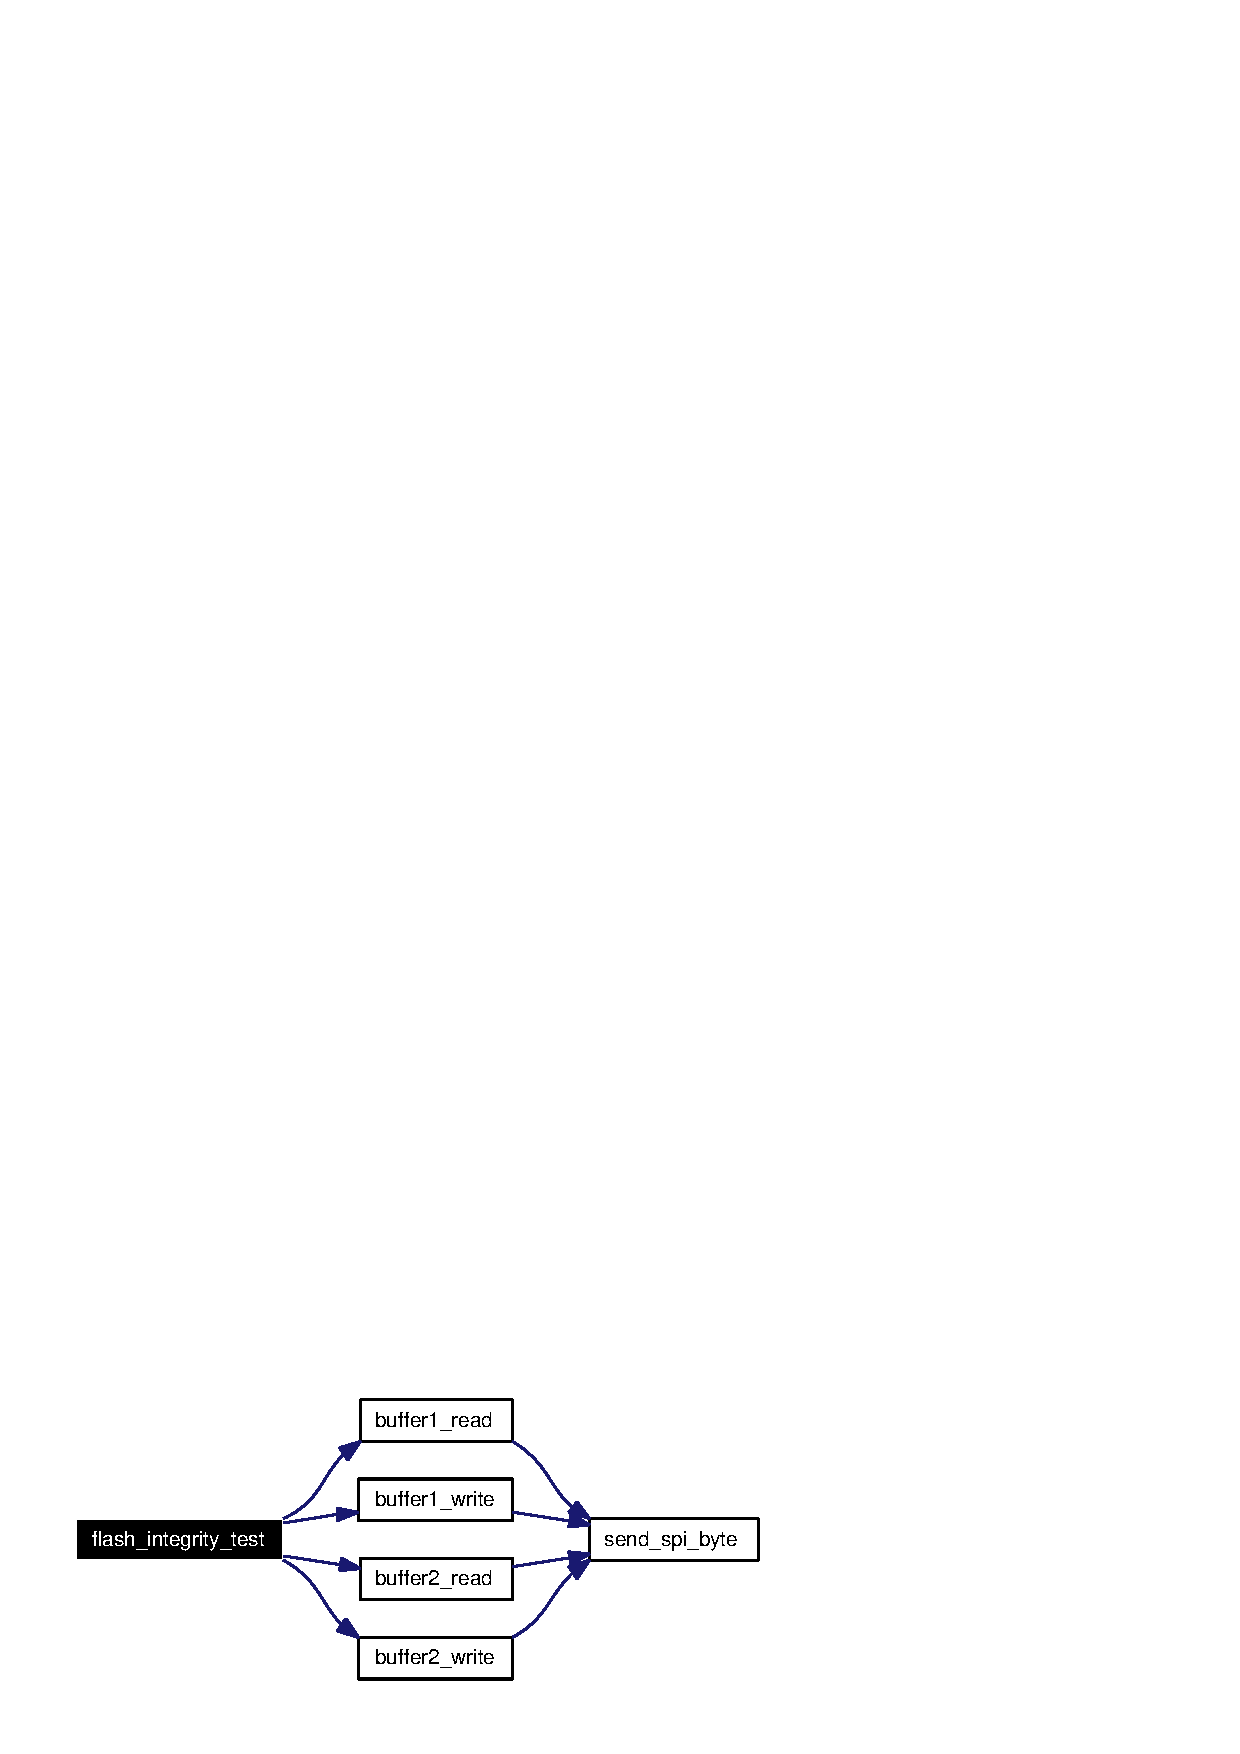
\includegraphics[width=182pt]{external__flash_8h_a4_cgraph}
\end{center}
\end{figure}
\index{external_flash.h@{external\_\-flash.h}!init_spi@{init\_\-spi}}
\index{init_spi@{init\_\-spi}!external_flash.h@{external\_\-flash.h}}
\subsubsection{\setlength{\rightskip}{0pt plus 5cm}void init\_\-spi (void)}\label{external__flash_8h_a6}


\index{external_flash.h@{external\_\-flash.h}!page_to_buffer1_compare@{page\_\-to\_\-buffer1\_\-compare}}
\index{page_to_buffer1_compare@{page\_\-to\_\-buffer1\_\-compare}!external_flash.h@{external\_\-flash.h}}
\subsubsection{\setlength{\rightskip}{0pt plus 5cm}void page\_\-to\_\-buffer1\_\-compare (unsigned {\em short})}\label{external__flash_8h_a9}




Definition at line 165 of file external\_\-flash.c.

References n\-CS\_\-HIGH, n\-CS\_\-LOW, and send\_\-spi\_\-byte().

\footnotesize\begin{verbatim}165                                                   {
166   unsigned char page_temp;
167   nCS_LOW;
168   send_spi_byte(0x60);           // command for byte write to buff 1
169   page_temp = (unsigned char)(page>>7);
170   send_spi_byte (page_temp);
171   page_temp = (unsigned char) (page<<1);
172   send_spi_byte (page_temp);
173   send_spi_byte (0x00);
174   nCS_HIGH;
175 }
\end{verbatim}\normalsize 




Here is the call graph for this function:\begin{figure}[H]
\begin{center}
\leavevmode
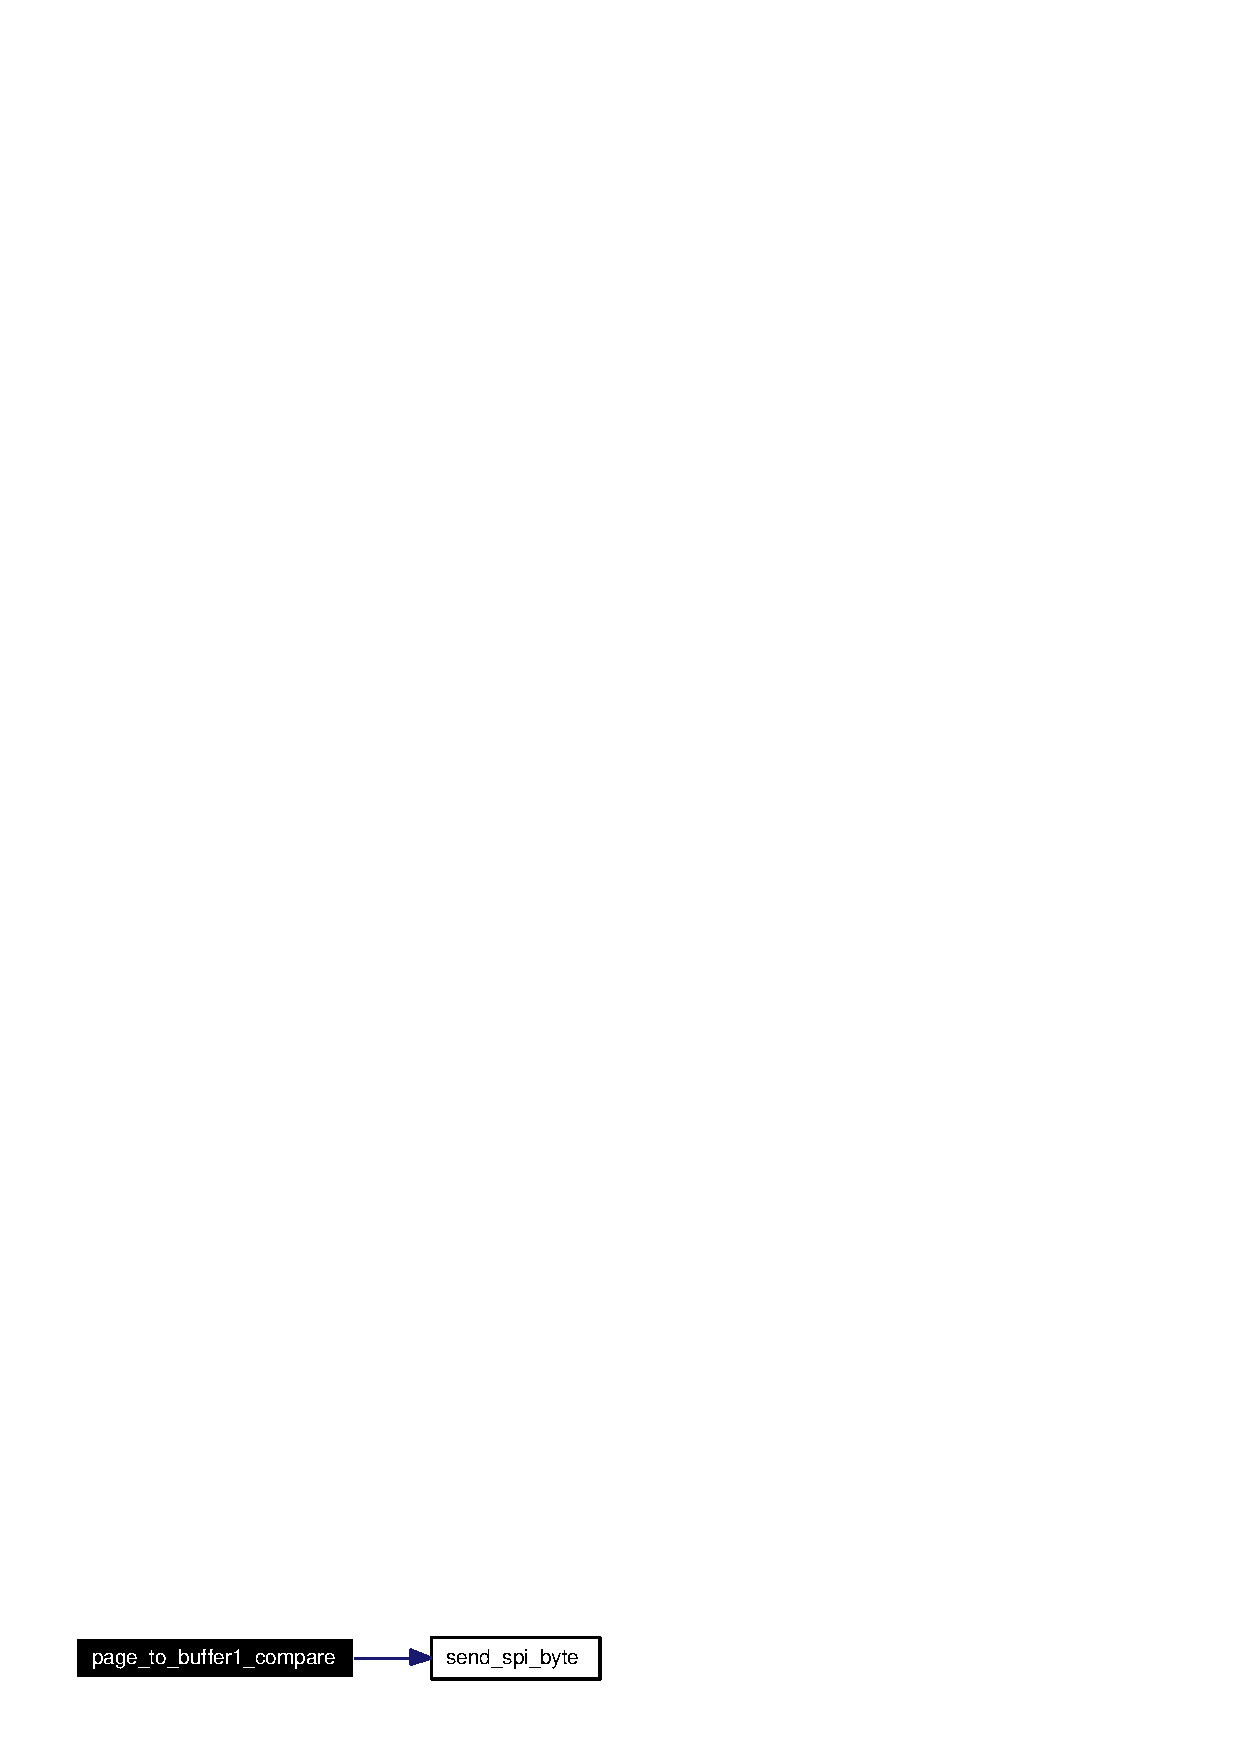
\includegraphics[width=144pt]{external__flash_8h_a9_cgraph}
\end{center}
\end{figure}
\index{external_flash.h@{external\_\-flash.h}!poll_status_register_blocking@{poll\_\-status\_\-register\_\-blocking}}
\index{poll_status_register_blocking@{poll\_\-status\_\-register\_\-blocking}!external_flash.h@{external\_\-flash.h}}
\subsubsection{\setlength{\rightskip}{0pt plus 5cm}unsigned char poll\_\-status\_\-register\_\-blocking (void)}\label{external__flash_8h_a12}




Definition at line 201 of file external\_\-flash.c.

References n\-CS\_\-HIGH, n\-CS\_\-LOW, and send\_\-spi\_\-byte().

\footnotesize\begin{verbatim}201                                                   {  
202   unsigned char status;
203   status = 0;
204   nCS_LOW;  
205   //  send_spi_byte(0x57);
206   send_spi_byte(0xD7);
207   while (!(status&0x80)) { 
208     status = send_spi_byte(0x00); // send data to get the spi to clock
209   }
210   nCS_HIGH;
211   return (status); 
212 }
\end{verbatim}\normalsize 




Here is the call graph for this function:\begin{figure}[H]
\begin{center}
\leavevmode
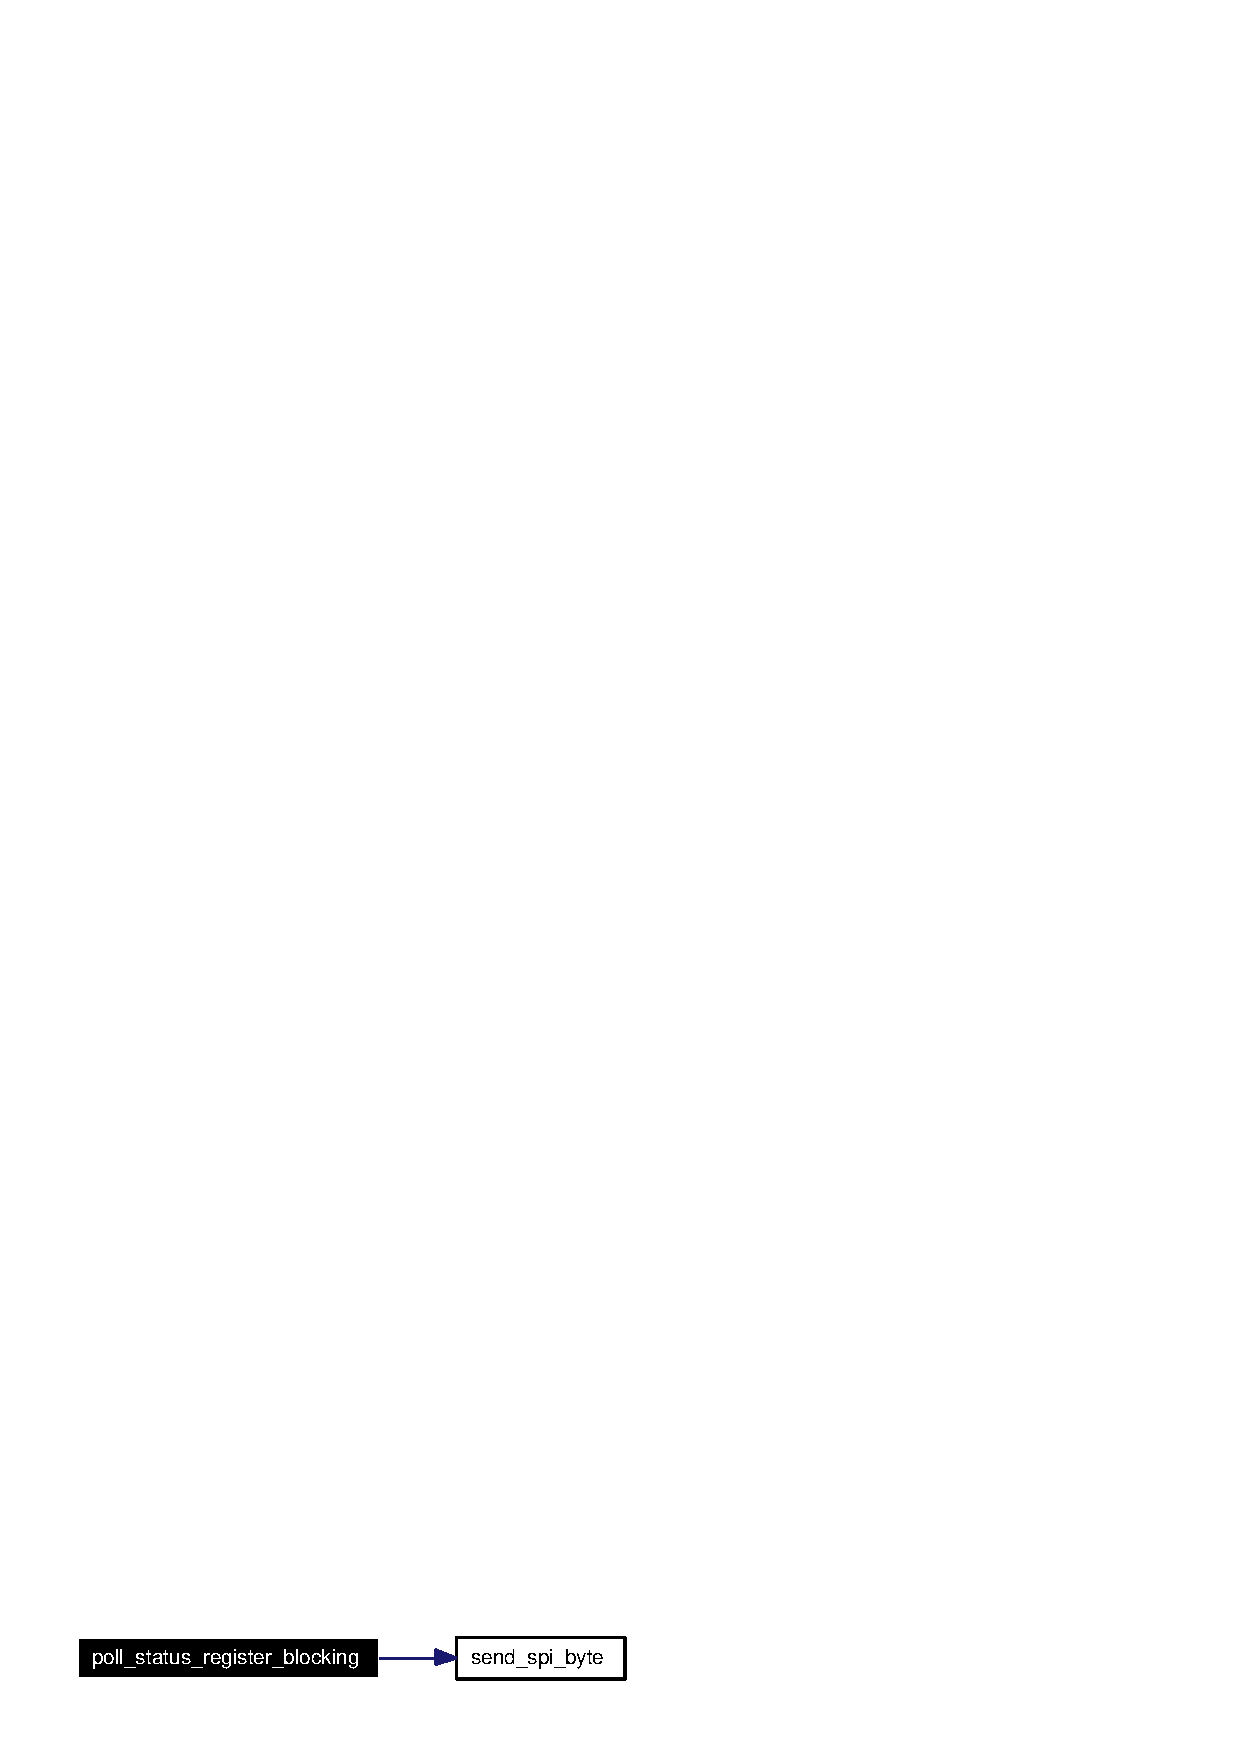
\includegraphics[width=150pt]{external__flash_8h_a12_cgraph}
\end{center}
\end{figure}
\index{external_flash.h@{external\_\-flash.h}!send_spi_byte@{send\_\-spi\_\-byte}}
\index{send_spi_byte@{send\_\-spi\_\-byte}!external_flash.h@{external\_\-flash.h}}
\subsubsection{\setlength{\rightskip}{0pt plus 5cm}unsigned char send\_\-spi\_\-byte (unsigned {\em char})}\label{external__flash_8h_a5}




Definition at line 154 of file ueaclib.c.

Referenced by buffer1\_\-read(), buffer1\_\-to\_\-page\_\-e(), buffer1\_\-write(), buffer2\_\-read(), buffer2\_\-to\_\-page\_\-e(), buffer2\_\-write(), init\_\-ueac\_\-state\_\-structure(), page\_\-to\_\-buffer1\_\-compare(), poll\_\-status\_\-register\_\-blocking(), start\_\-main\_\-array\_\-read(), and write\_\-dac().

\footnotesize\begin{verbatim}154                                                      {
155   TXBUF0 = data_byte;        // buffer 1 write  
156   while(!(UTCTL0&0x01));     // wait until transmitter empty
157   return(RXBUF0);            // return any received data
158                              // No data returned from DAC
159                              // SPI flash returns read data
160 }
\end{verbatim}\normalsize 


\index{external_flash.h@{external\_\-flash.h}!start_main_array_read@{start\_\-main\_\-array\_\-read}}
\index{start_main_array_read@{start\_\-main\_\-array\_\-read}!external_flash.h@{external\_\-flash.h}}
\subsubsection{\setlength{\rightskip}{0pt plus 5cm}void start\_\-main\_\-array\_\-read (unsigned {\em short}, unsigned {\em short})}\label{external__flash_8h_a7}




Definition at line 137 of file external\_\-flash.c.

References n\-CS\_\-LOW, and send\_\-spi\_\-byte().

Referenced by init\_\-ueac\_\-state\_\-structure().

\footnotesize\begin{verbatim}137                                                                     {
138   unsigned char page_temp; 
139 
140   nCS_LOW;
141   // opcode
142   send_spi_byte(0xE8);  // SPI Mode 0 or 3  
143 
144   // Prepare/send the page and address fields
145   page_temp = (unsigned char)(page>>7);
146   send_spi_byte (page_temp);
147   page_temp = (unsigned char) (page<<1);
148   if (addr>0xff) {
149     page_temp |=0x01;
150   }
151   send_spi_byte (page_temp);
152   send_spi_byte ((unsigned char) addr);
153 
154   // additional bytes
155   send_spi_byte(0x00);
156   send_spi_byte(0x00);
157   send_spi_byte(0x00);
158   send_spi_byte(0x00);
159 }
\end{verbatim}\normalsize 




Here is the call graph for this function:\begin{figure}[H]
\begin{center}
\leavevmode
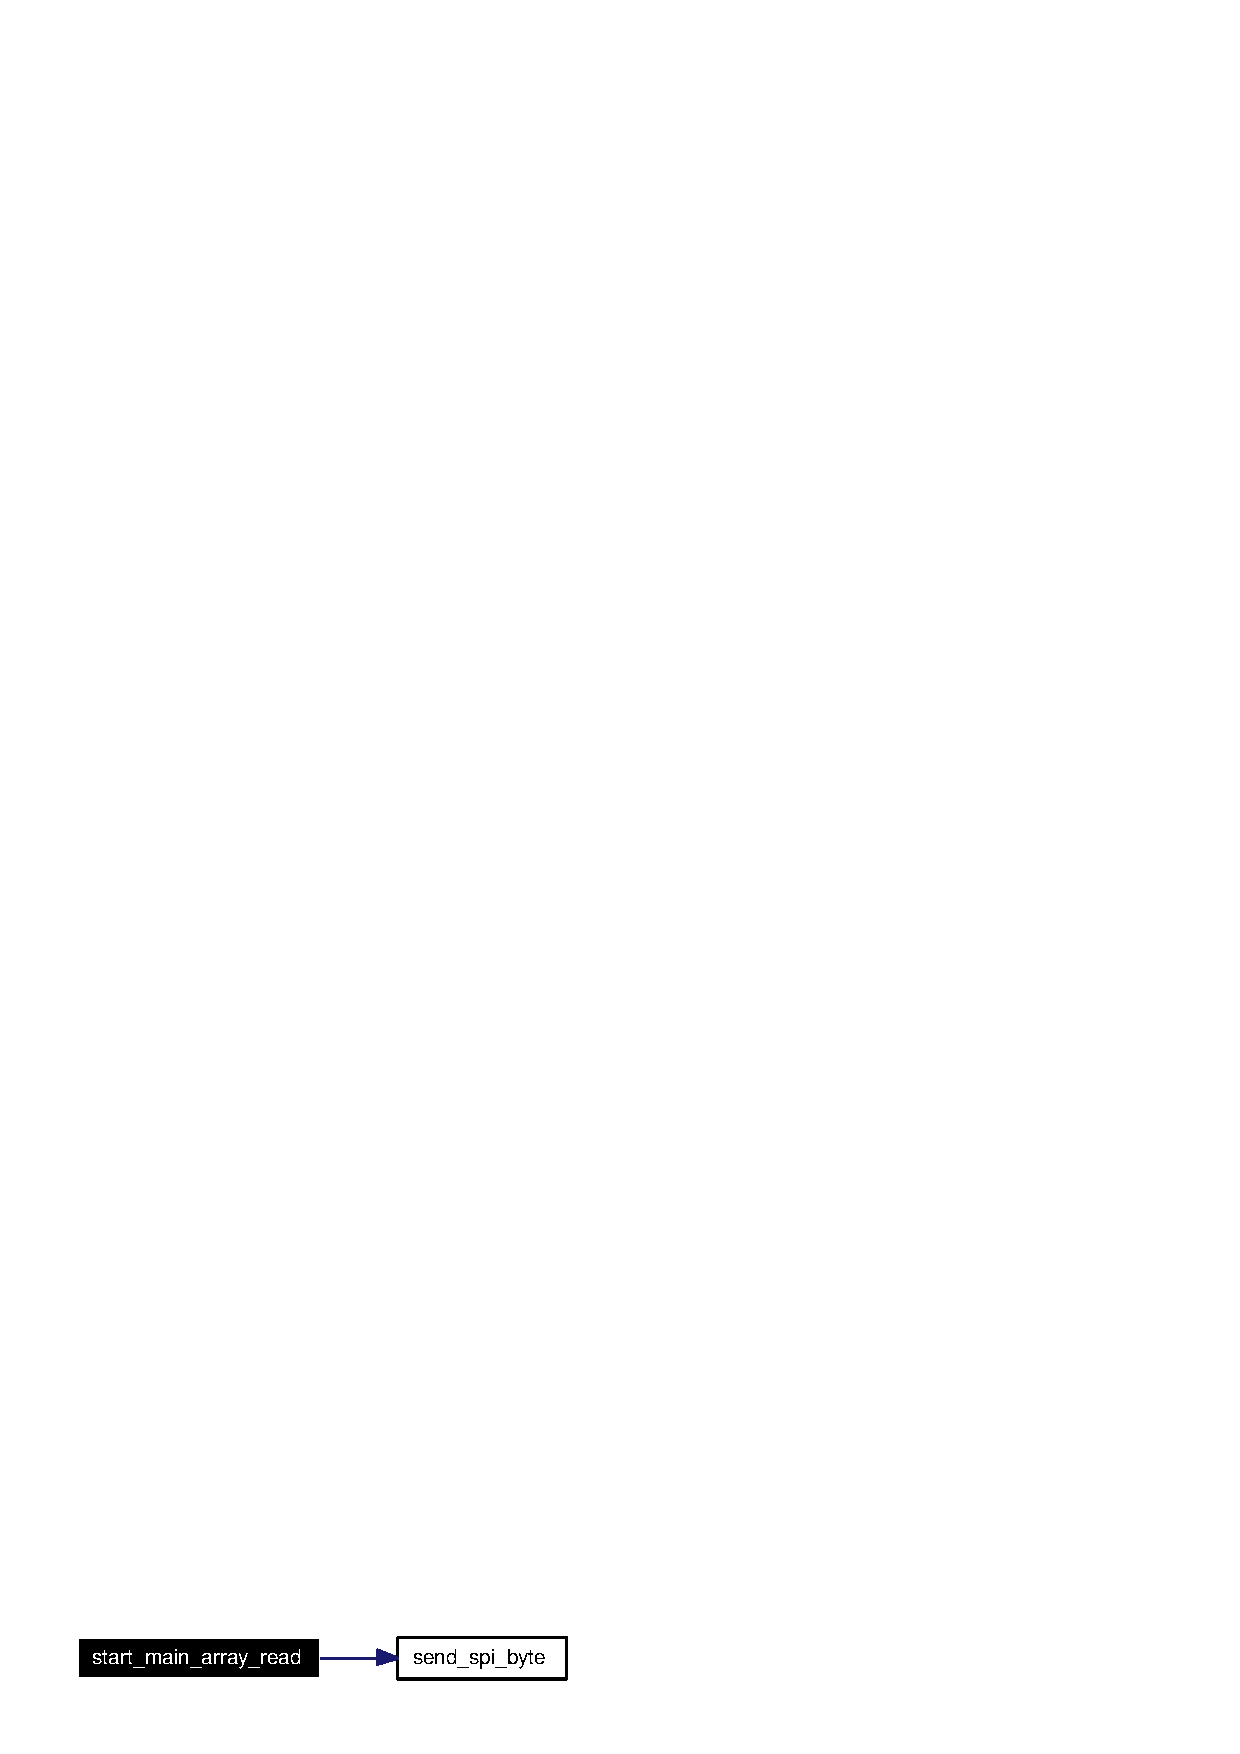
\includegraphics[width=136pt]{external__flash_8h_a7_cgraph}
\end{center}
\end{figure}
